\documentclass[a4paper 12pt]{article}

\usepackage[utf8]{inputenc}
\usepackage[T1]{fontenc}
\usepackage{mathptmx}
\usepackage{textcomp}
\usepackage[UKenglish]{babel}
\usepackage{amsmath, amssymb}
\usepackage{float}
\usepackage{xcolor}
\definecolor{codegreen}{rgb}{0,0.6,0}
\definecolor{codepurple}{rgb}{0.58,0,0.82}
\usepackage{listings}
\lstdefinestyle{code}{
	commentstyle=\color{codegreen},
	keywordstyle=\color{magenta},
	stringstyle=\color{codepurple},
	showspaces=false,
	showstringspaces=false,
	breaklines=true
}
\lstset{style=code}
\usepackage[hidelinks]{hyperref}
\hypersetup{
	colorlinks=false
}
\usepackage[style=ieee]{biblatex}
\bibliography{sources/biblio}
\renewcommand{\baselinestretch}{1.5}

\setlength{\parindent}{0pt}
\setlength{\parskip}{1em}

% figure support
\usepackage{import}
\usepackage{xifthen}
\pdfminorversion=7
\usepackage{pdfpages}
\usepackage{transparent}
\newcommand{\incfig}[1]{%
	\def\svgwidth{\columnwidth}
	\import{./figures/}{#1.pdf_tex}
}

\pdfsuppresswarningpagegroup=1

\begin{document}
\hypersetup{pageanchor=false}
\begin{titlepage}
  \begin{center}

    \textsc{\LARGE Dublin City University}\\[1cm]
    \textsc{\Large Electronic and Computer Engineering}\\[0.5cm]

    {\LARGE \bfseries Title\\[0.4cm]}
    {\Large \bfseries Subtitle\\[0.4cm]}

    \begin{figure}[H]
	
\includegraphics{images/Dcu-logo.png}
	\centering
    \end{figure}

    \vskip 2cm
    \emph{Author}\\[0.1cm]
    \noindent\makebox[\textwidth]{%
      \begin{tabular}{ll}%
        Michael Lenehan & michael.lenehan4@mail.dcu.ie \\
	Student Number: & 15410402 \\
    \end{tabular}}\\[0.1cm]

    \vfill

    % Bottom of the page
    % Probably replaced with date of deadline
    {\large{xx/xx/20xx}}

  \end{center}
\end{titlepage}

\hypersetup{pageanchor=true}
\pagenumbering{alph}
\thispagestyle{plain}
\begingroup
\renewcommand{\cleardoublepage}{}
\renewcommand{\clearpage}{}

\LARGE{Declaration}

\endgroup

\vskip 1cm

I declare that this material, which I now submit for assessment, is entirely my
own work and has not been taken from the work of others, save and to the extent
that such work has been cited and acknowledged within the text of my work. I
understand that plagiarism, collusion, and copying are grave and serious
offences in the university and accept the penalties that would be imposed should
I engage in plagiarism, collusion or copying. I have read and understood the
Assignment Regulations set out in the module documentation. I have identified
and included the source of all facts, ideas, opinions, and viewpoints of others
in the assignment references. Direct quotations from books, journal articles,
internet sources, module text, or any other source whatsoever are acknowledged
and the source cited are identified in the assignment references. This
assignment, or any part of it, has not been previously submitted by me or any
other person for assessment on this or any other course of study.

I have read and understood the DCU Academic Integrity and Plagiarism at
\url{https://www4.dcu.ie/sites/default/files/policy/1%20-%20integrity\_and\_plagiarism\_ovpaa_v3.pdf}
and IEEE referencing guidelines found at
\url{https://loop.dcu.ie/mod/url/view.php?id=448779}.

\vskip 1cm
Signed: \underline{\ \ \ \ \ \ \ \ \ \ \ \ \ \ \ \ \ \ \ \ \ \ \ \ \ \ \ \ \ \ \
\ \ \ \ \ \ } \hspace{20mm}Date: \underline{10/04/2020}

\hspace*{0mm}\phantom{Signed:}Michael Lenehan

\pagebreak

\pagenumbering{arabic}
\tableofcontents
\clearpage
\section{Introduction}
The Red-Black Tree is an implementation of the Binary Search Tree which
maintains balance. Nodes of a Red-Black tree are either coloured red or black,
hence the name. By ensuring that there are never two directly connected red
nodes, rotate operations ensure that the tree is always balanced.

The concept for this type of binary search tree was instroduced by Rudolf Bayer
in 1972\cite{wpedia}. They are particularly useful in real-time applications, and as such
were included in the implementation of the ``Completely Fair Scheduler'' in the
Linux Kernel in version 2.6.23.

The main advantage of using Red-Black trees is the time complexity. Red-Black
trees have a time complexity of O(logN) for insertion and deletion operations,
improving upon the typical complexity of O(N) for more basic Binary Search Tree
implementations\cite{wpedia}.

For each node in a tree there is a set colour, up to one parent node, and up to
two child nodes. The root node if a red-black tree is always coloured black,
along with any null nodes (i.e. empty/leaf nodes). Two red nodes can not be
directly connected\cite{geeksIntro}. Each left child node in a tree must
have a value less than the parent node, and each right child node in a tree must
have a value greater than the parent node. Maintaining balance within the tree
means that the case of the root node being the lowest value in a constantly
incrementing tree, i.e. all child nodes are in the right branch, cannot occur.
This balancing means that the time complexity of traversing the tree does not
increase past O(logN).

\section{Red-Black Tree Operation}
The main feature of a red-black tree is it's ability to maintain balance. It
does this through a number of operations. On adding a new value to to tree, an
Insertion operation is used to define where within the tree the new value will
be placed. On deleting a value from the tree, the tree must be restructured in
order to allow any child node of the deleted node to remain connected to the
rest of the tree. Recoloring is a technique which is unique to Red-Black Trees,
and allows for a tree to be rebalanced without using a rotation operation. If
recoloring is not successful, rotations are used following these operations to
ensure that balance is maintained within the tree.

\subsection{Insertion}

Insertions are done based on the value of the incoming node. The incoming node
value is compared agains the root node value. If the incoming node value is
greater than the root node value, the comparison is repeated with the root nodes
right child node. If the incoming node value is less than the root nodes value,
the comparison is repeated with the root nodes left child node\cite{geeksInsert}
. This operation
is typically called recursively in order to traverse the tree until the point
that there is no left or right child node with which to compare, at which point
the incoming node can be placed in the tree.

Following the insertion of the incoming node to the tree, the tree must be
rebalanced. This is to maintain the traversal speed of the tree. Rebalancing is
done via either recoloring or rotation, as described below.

\subsection{Deletion}

Deletion within a Red-Black tree involves removing the specified value from the
tree. The specified value is compared to the root node value, and, if greater
than the root node value, a comparison is made with the right child node value,
and if less than the root node value, a comparison is made with the left child
node value. This operation is called recursively until the specified node value
is found. This node is then deleted from the tree.

If the specified node value is a leaf node, or a node with one child, then this
deletion is relatively simple. If the node has one child, then the child node
replaces the deleted node within the tree and a recolouring or rotation must be
performed. If the node has no children, i.e. is a leaf node, then the node is
simply deleted\cite{geeksDelete}.

For any node deletion in which the specified node is not a leaf node, or a node
with only one child, i.e. the specified node is ``internal'', the order of all
child nodes must be retained, and after deletion must be reordered into the
existing tree\cite{geeksDelete}. This is, therefore, a much more complex operation.

\subsection{Tree Balancing}

Tree balancing is required in order to maintain the traversal time complexity
within a red-black tree. The two techniques used in tree balancing are
``Recoloring'' and ``Rotation''. Recoloring involves changing the colours
associated with the nodes in the tree, whereas rotation involves moving the
nodes of the tree, replacing the existing root node.

\subsubsection{Recoloring}

There are a number of cases for recoloring of nodes within a red-black tree. As
the root node is required to be black, and two red nodes cannot be adjacent,
the recoloring must be done in such a way as to maintain these rules.

Any new node being inserted to the tree is initially coloured red. The parent
node colour is then checked. If this node is red, the rule stating that two red
nodes cannot be directly connected is being violated. The parent node color is
changed to black, and the colour of the parents parent (i.e. the grandparent),
is changed to red. Following this, rotations may be required to make a valid
red-black tree, for example if the grandparent node is the root of the tree
(which must be black)\cite{geeksInsert}.

\subsubsection{Rotation}

Rotations are used within the red-black tree to rebalance the tree without
modifying the overall order of the elements in the tree. When a node is
inserted, recoloring is first performed, however, if this does not result in a
valid, balaced, red-black tree, a rotation operation must be completed.

Following recolouring, if the root node is red, a left or right rotation must
occur. If the newly added node is in the left branch, a right rotation occurs,
and if in the right branch, a left rotation occurs\cite{geeksInsert}.
These rotations may be
requied to be done recursively in order to acquire a valid and balanced red-black tree.

\section{Red-Black Tree Code}
The aim of the code portion of this assignment is to implement a Red-Black Tree
which can store paired ``finish number'' and ``VPN'' values. The Red-Black Tree
is required to sort the pairs by finish number. In order to ensure that the code
is working as intended, 100 input pairs must be inserted to the tree, with the
original input pairs and the tree following all insertions being printed to
verify its operation.

Provided for the purposes of the coding section of this assignment were a
selection of random number generating functions, along with an implementation of
a red-black tree\cite{zentut} which needs to be modified. The red-black tree
implementation
takes integer values for its elements, however, the output from the random
number generator is of type long. The required implementation must also be able
to perform insertions of two values.

In order to store both the ``finish key'' and the ``vpn'' values, a C structure
named ``node\_entry'' was defined in the ``node\_entry.h'' file. In this header
file, the finish key is defined as an unsigned long, while the vpn is defined as
an unsigned int. A function to display the values of the struct is defined
within this header file, and is implemented within the ``node\_entry.c'' file.

\begin{figure}[H]
	\centering
	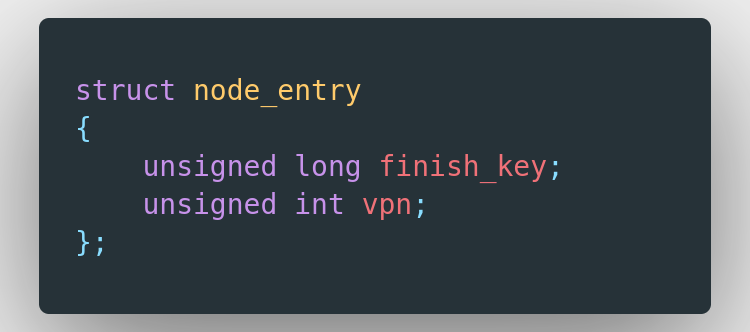
\includegraphics[width=0.8\textwidth]{images/nodeEntry}
	\caption{Node Entry Structure}
	\label{fig:images-nodeEntry}
\end{figure}

Within the ``redblack.h'' file, the type definition for ``ElementType'' must be
changed from type int to type ``struct node\_entry''. This allows for the finish
key/vpn pairs to be passed in as arguements to the functions of the red-black
tree, such as insertion etc.

\begin{figure}[H]
	\centering
	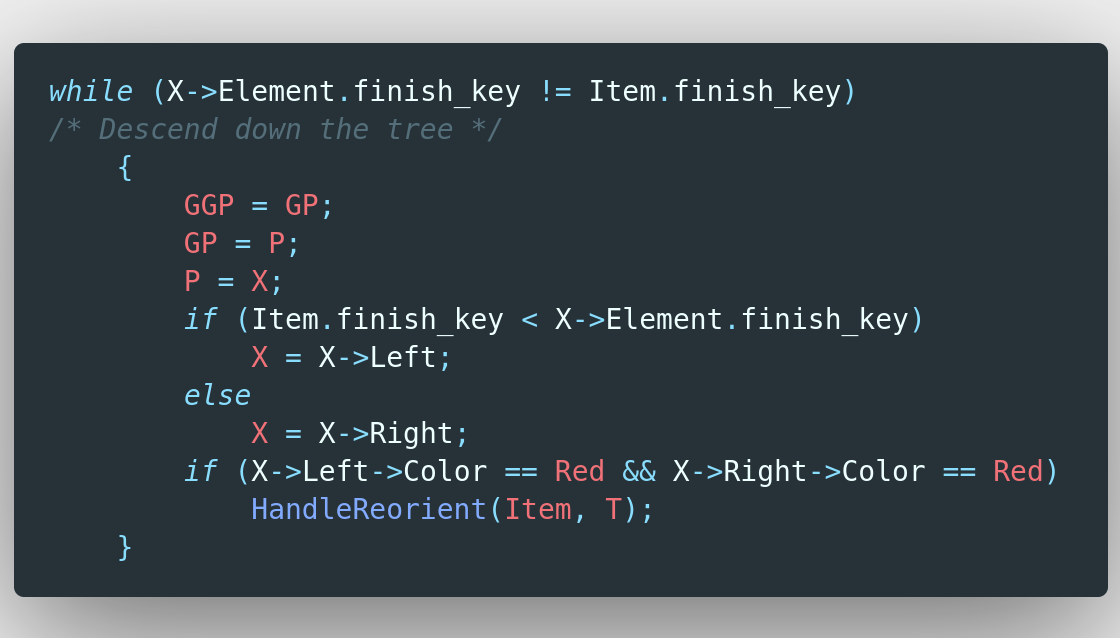
\includegraphics[width=0.8\textwidth]{images/example}
	\caption{Example of Modifications to the Red-Black Tree Code}
	\label{fig:images-ex}
\end{figure}

Within the ``redblack.c'' file, all references to ``Element'', which is the
value in the tree, must be replaced with ``Element.finish\_key''. This allows
for all sorting within the tree to be done based on the finish key, rather than
on the vpn. The return type of the ``Retrieve'' function must also be changed to
``long'', as it is no longer returning an integer value, rather the value of the
finish key, which is long.

Within the main function, the tree and random number generator are both
initialized. The tree is initialized as an empty red-black tree, and the random
number generator is initialised with the seeds (0, 0, 1541, 0402). Within the
``init'' function, the seeds are set to (1, 2, 3, 4). An empty array of type
node\_entry is defined, with a size of 100. A loop iterates from 0 to
100, populating the finish key values with random long values from 0-999, using
the ``fairdie'' function. The vpn values are populated with the iteration value,
i.e. 0-99. Within this loop, each new node\_entry item is inserted into the tree
using the ``Insert'' function. The ``PrintTree'' function is then used in order
to print the sorted contents of the tree, which verifies the correct operation
of the tree.

\section{Conclusion}
Red-Black Trees offer traversal time complexity in the order O(logN). While the
implementation may be complex, the benefits of the red-black tree are clear, and
its benefits in real-time applications are why it was included in the Linux
Kernel's ``Completely Fair Scheduler''.

The red-black tree code shows how the tree can be used to sort values, while
maintaining balance, and the time complexity of the tree. An issue was
experienced in the code, when using the randomly generated numbers the tree
would overwrite each number in the tree with the last input number, resulting in
only one number (the final input number) in the completed tree. As no changes
were made to the structure of the tree's code, this issue was unable to be
resolved.

\clearpage
\printbibliography
\end{document}
